\documentclass[../Cours.tex]{subfiles}

\begin{document}
\clearpage
\thispagestyle{empty}

\color{black}
\addcontentsline{toc}{section}{\textcolor{vert}{Corrigé}}%

\begin{center}
    \Huge{Épreuve commune de $4^{\mbox{ème}}$ (entraînement)}
\end{center}

\begin{questions}

\exercice
Chaque question ne contient \textbf{qu'une seule bonne réponse}, et ne nécessite \textbf{aucune justification}.

\begin{center}
\begin{tabularx}{\linewidth}{|l|C|C|C|C|} \hline
    Question & A & B & C & D \\\hline \hline 
    \makecell[l]{Dans laquelle de ces figures les \\deux droites sont parallèles ?}
    & 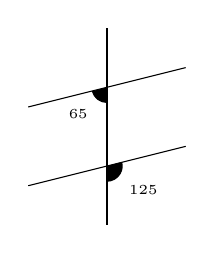
\begin{tikzpicture}
        \draw (0,0) -- (2,0.5);
        \draw (0,-1) -- (2,-0.5);
        \draw (1,1) -- (1,-1.5);
        \fill[black] (1,-0.75) -- ++(0,-0.2) arc(-90:15:0.2) node[midway,below right]{\tiny{\ang{125}}} -- cycle;
        \fill[black] (1,0.25) -- ++(0,-0.2) arc(-90:-165:0.2) node[midway,below left]{\tiny{\ang{65}}} -- cycle;
    \end{tikzpicture}
    &   \cellcolor{green} 
    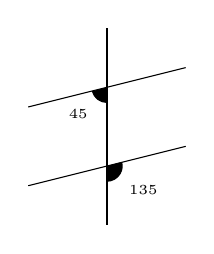
\begin{tikzpicture}
        \draw (0,0) -- (2,0.5);
        \draw (0,-1) -- (2,-0.5);
        \draw (1,1) -- (1,-1.5);
        \fill[black] (1,-0.75) -- ++(0,-0.2) arc(-90:15:0.2) node[midway,below right]{\tiny{\ang{135}}} -- cycle;
        \fill[black] (1,0.25) -- ++(0,-0.2) arc(-90:-165:0.2) node[midway,below left]{\tiny{\ang{45}}} -- cycle;
    \end{tikzpicture}
    & 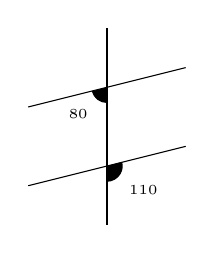
\begin{tikzpicture}
        \draw (0,0) -- (2,0.5);
        \draw (0,-1) -- (2,-0.5);
        \draw (1,1) -- (1,-1.5);
        \fill[black] (1,-0.75) -- ++(0,-0.2) arc(-90:15:0.2) node[midway,below right]{\tiny{\ang{110}}} -- cycle;
        \fill[black] (1,0.25) -- ++(0,-0.2) arc(-90:-165:0.2) node[midway,below left]{\tiny{\ang{80}}} -- cycle;
    \end{tikzpicture}
    & 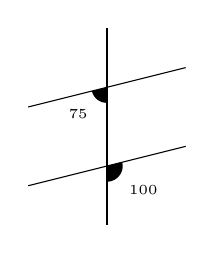
\begin{tikzpicture}
        \draw (0,0) -- (2,0.5);
        \draw (0,-1) -- (2,-0.5);
        \draw (1,1) -- (1,-1.5);
        \fill[black] (1,-0.75) -- ++(0,-0.2) arc(-90:15:0.2) node[midway,below right]{\tiny{\ang{100}}} -- cycle;
        \fill[black] (1,0.25) -- ++(0,-0.2) arc(-90:-165:0.2) node[midway,below left]{\tiny{\ang{75}}} -- cycle;
    \end{tikzpicture} \\\hline
    \makecell[l]{Lequel de ces nombres \\n'est pas divisible par 9 ?} & \cellcolor{green} 784 &  4995 & 1566 & 88884 \\\hline
    \makecell[l]{Deux amis ont joué au loto et leur mise \\s’est faite selon le ratio 3:5. \\Ils gagnent 64 euros. Quelle est la somme\\d’argent qui revient à chacun d’eux ?} & \qty{3}{\EURO} et \qty{5}{\EURO} & \cellcolor{green} \qty{24}{\EURO} et \qty{40}{\EURO} & \qty{40}{\EURO} et \qty{24}{\EURO} & \qty{5}{\EURO} et \qty{3}{\EURO} \\\hline
    \makecell[l]{Soit la série de nombres \{15 ; 10 ; 13 ; 9 ; 10\}\\ La moyenne de la série est ...} & \num{11.2} &\cellcolor{green}  \num{11.4} & \num{11.6} & \num{11.8} \\\hline
\end{tabularx}
\end{center}

{
    \color{rouge}
    \questionX
    
    \begin{tikzpicture}
        \draw[noir] (0,0) -- (2,0.5);
        \draw[noir] (0,-1) -- (2,-0.5);
        \draw[noir] (1,1) -- (1,-1.5);
        \fill[noir] (1,-0.75) -- ++(0,-0.2) arc(-90:15:0.2) node[midway,below right]{\tiny{\ang{135}}} -- cycle;
        \fill[noir] (1,0.25) -- ++(0,-0.2) arc(-90:-165:0.2) node[midway,below left]{\tiny{\ang{45}}} -- cycle;
    \end{tikzpicture}
    
    La somme des mesures des deux angles noirs doit être égale à \ang{180}. 
    
    Sur le schéma ci-dessous, les angles rouge et vert sont \emph{correspondants}. Par conséquent, s'ils ont la même mesure, alors les droites sont parallèles et \emph{vice versa}. 
    
    De plus les angles rouge et bleu sont supplémentaires, autrement dit la somme de leur mesure vaut \ang{180}.

    \begin{tikzpicture}
        \draw[noir] (0,0) -- (2,0.5);
        \draw[noir] (0,-1) -- (2,-0.5);
        \draw[noir] (1,1) -- (1,-1.5);
        \fill[vert] (1,-0.75) -- ++(0,-0.2) arc(-90:15:0.2) node[midway,below right]{\tiny{\ang{135}}} -- cycle;
        \fill[red] (1,0.25) -- ++(0,-0.2) arc(-90:15:0.2) node[midway,below right]{\tiny{\ang{135}}} -- cycle;
        \fill[bleu] (1,0.25) -- ++(0,-0.2) arc(-90:-165:0.2) node[midway,below left]{\tiny{\ang{45}}} -- cycle;
    \end{tikzpicture}

    \questionX Pour savoir si un nombre est divisible par 9, on calcule la somme des chiffres, et on vérifie si elle se trouve dans la table de 9.
    \begin{itemize}
        \item $784 \longrightarrow 7+8+4 = 19$ (pas divisible par 9)
        \item $4995 \longrightarrow 4+9+9+5 = 27$ ($27 = 9\times 3$)
        \item $1566 \longrightarrow 1+5+6+6 = 18 $ ($18 = 9 \times 2$)
        \item $88884 \longrightarrow 8+8+8+8+4 = 36$ ($36 = 9 \times 4$)
    \end{itemize}

    \questionX 64 euros dans le ratio 3:5. Cela signifie que l'on va répartir les 64 euros en 8 morceaux ($3+5=8$), en donner 3 à la première personne et 5 à la deuxième.

    1 morceau correspond à $\frac{\qty{64}{\EURO}}{8} = \qty{8}{\EURO}$.

    Donc 3 morceaux correspondent à $3 \times 8 = \qty{24}{\EURO}$ et les 5 morceaux correspondent à $5 \times 8 = \qty{40}{\EURO}$.

    \questionX Pour calculer la moyenne de ces 5 valeurs, on calcule leur somme, et on divise le résultat obtenu par le nombre de valeurs de cette série statistique à savoir 5. Cela donne : 
    \[
        \frac{15+10+13+9+10}{5} = \frac{57}{5} = \num{11.4}
    \]
}

\exercice
Sur la figure ci-dessous, $C$ est un point du demi-cercle de diamètre $[PR]$ tel que $CR=\qty{1500}{\milli\metre}$. Le triangle $RCP$ est rectangle en $C$.

\begin{centre}
    \begin{tikzpicture}[scale=1.5]
        \draw (-1.5,0) arc(180:0:1.5);
        \draw (-1.5,0) node[left]{$R$} -- ({1.5*cos(120)},{1.5*sin(120)}) node[above left]{$C$} -- (1.5,0) node[right]{$P$} -- cycle;
        \draw[Latex-Latex] (-1.5,-0.15) -- +(3,0) node[midway,below]{\qty{3000}{\milli\metre}};
        \fill[black,rotate around={-120:({1.5*cos(120)},{1.5*sin(120)})}] ({1.5*cos(120)},{1.5*sin(120)}) rectangle +(0.1,0.1);
    \end{tikzpicture}
\end{centre}

\question Calculer la distance $PC$.

{\color{rouge}

Le triangle $RCP$ est rectangle en C. Son hypoténuse est $[RP]$.

D'après le théorème de Pythagore
\begin{align*}
    RP^2 &= RC^2 + CP^2 \\
    PC^2 &= RP^2 - RC^2 \\
    PC^2 &= \num{3000}^2 - \num{1500}^2 \\
    PC^2 &= \num{9000000} - \num{2250000} \\
    PC^2 &= \num{6750000} \\
    \Aboxed{PC &= \sqrt{\num{6750000}}~\unit{\milli\metre}} \longleftarrow \mbox{valeur exacte} \\
    PC &\approx \qty{2598}{\milli\metre} \longleftarrow \mbox{valeur approchée}
\end{align*}
}

\question En déduire l'aire du triangle $RCP$.

{\color{rouge}
\begin{mdframed}
    Pour calculer l'aire d'un triangle, on utilise la formule $\frac{\mbox{base} \times \mbox{hauteur}}{2}$. 
    %
    En particulier, dans un triangle rectangle, la base et la hauteur peuvent correspondre aux 2 côtés de l'angle droit. 
\end{mdframed}
\begin{align*}
    \curs{A} &= \frac{\mbox{base} \times \mbox{hauteur}}{2} \\
    &= \frac{RC \times RP}{2} \\ 
    &= \frac{\qty{1500}{\milli\metre} \times \sqrt{6750000}~\unit{\milli\metre} }{2} \\ 
    \Aboxed{\curs{A}&\approx \qty{1948557}{\milli\metre\squared}} \longleftarrow \mbox{valeur approchée}\\ 
\end{align*}
}


\exercice
Voici un programme de calcul.

\begin{center}
    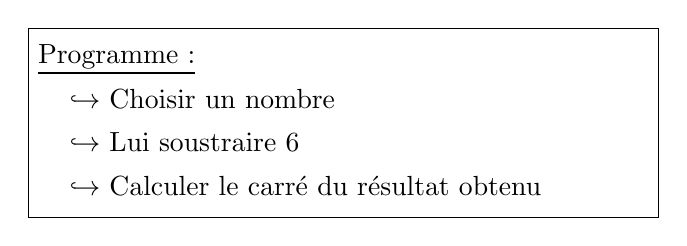
\begin{tikzpicture}
        \draw (0,0.5) rectangle +(8,2.4);
        \node[anchor=west] at (0,2.5) {\underline{Programme :}};
        \node[anchor=west] at (0.4,2) {$\hookrightarrow$ Choisir un nombre};
        \node[anchor=west] at (0.4,1.45) {$\hookrightarrow$ Lui soustraire 6};
        \node[anchor=west] at (0.4,0.9) {$\hookrightarrow$ Calculer le carré du résultat obtenu};
    \end{tikzpicture}
\end{center}

\question Si on choisit le nombre 4 au départ, montrer que le résultat obtenu est 4.

{\color{rouge}
    \begin{itemize}
        \item Choisir un nombre $\longrightarrow$ $4$
        \item Lui soustraire 6 $\longrightarrow$ $4-6 = -2$
        \item Calculer le carré du résultat $\longrightarrow$ $(-2)^2 = \boxed{4}$
    \end{itemize}
}

\question On choisit 15 comme nombre de départ, quel est le résultat obtenu ?

{\color{rouge}
    \begin{itemize}
        \item Choisir un nombre $\longrightarrow$ $15$
        \item Lui soustraire 6 $\longrightarrow$ $15-6 = 9$
        \item Calculer le carré du résultat $\longrightarrow$ $9^2 = \boxed{81}$
    \end{itemize}
}

\question Si, en réalisant le programme, on obtient 144, quel nombre a-t-on choisi au départ ?

{\color{rouge}
On va réaliser le programme de calcul à l'envers.
    \begin{itemize}
        \item Le résultat $\longrightarrow$ $144$
        \item Calculer la racine carrée du résultat $\longrightarrow$ $\sqrt{144} = 12$
        \item Ajouter 6 $\longrightarrow$ $12+6 = \boxed{18}$
    \end{itemize}
}

\question 
    \subquestion Réaliser le programme en choisissant $x$, quelle expression littérale obtient-on ?

    {\color{rouge}
    \begin{itemize}
        \item Choisir un nombre $\longrightarrow$ $x$
        \item Lui soustraire 6 $\longrightarrow$ $x-6$
        \item Calculer le carré du résultat $\longrightarrow$ $\boxed{(x-6)^2}$
    \end{itemize}
    }
    
    \subquestion Montrer que cette expression littérale est aussi égale à $x^2-12x+36$.

    {\color{rouge}
    \begin{align*}
        (x-6)^2 &= (x-6)(x-6) \\ 
        &= x \times x + x \times (-6) + (-6) \times x + (-6) \times (-6) \\
        &= x^2 - 6x - 6x + 36 \\
        \Aboxed{(x-6)^2 &= x^2 -12x + 36}
    \end{align*}
    }

\exercice
Mathilde est une élève de quatrième qui mesure \qty{1.55}{\metre} et qui souhaite déterminer la hauteur d'un cocotier. Elle a vu en cours de mathématiques que l'on pouvait utiliser son ombre pour calculer la hauteur d'un objet trop grand pour les outils classiques.\\ 

Dans la figure ci-dessous, les points $B$, $D$ et $C$ sont alignés, et les points $B$, $E$, $A$ sont alignés.

\begin{center}
    \begin{tikzpicture}[scale=1.4]
        \coordinate (A) at (0,0);
        \coordinate (B) at (7,0);
        \coordinate (C) at (0,3);
        \coordinate (D) at ($(B)!0.5!(C)$);
        \coordinate (E) at ($(B)!(D)!(A)$);
        \draw (A) -- (B) -- (C) -- cycle;
        \draw (D) -- (E);
        \node[left] at (A) {$A$};
        \node[right] at (B) {$B$};
        \node[left] at (C) {$C$};
        \node[above] at (D) {$D$};
        \node[below] at (E) {$E$};
        \draw[Latex-Latex] ($(A)+(0,-0.2)$) -- ($(E)+(-0.2,-0.2)$) node[midway,below]{\qty{7}{\metre}};
        \draw[Latex-Latex] ($(E)+(0.2,-0.2)$) -- ($(B)+(-0.2,-0.2)$) node[midway,below]{\qty{3}{\metre}};
        \node[above,rotate=90] at ($(A)!0.5!(C)$) {cocotier};
        \draw[Latex-Latex] (C) ++(-0.5,0) -- ++(0,-3) node[midway,left]{?};
        \node[above,rotate=90] at ($(D)!0.5!(E)$) {Mathilde};
    \end{tikzpicture}
\end{center}

\question Calculer la hauteur du cocotier.

{\color{rouge}
\begin{itemize}
    \item Les points B, E et A sont alignés
    \item Les points B, D et C sont alignés
    \item Le cocotier et Mathilde sont à la verticale par rapport au sol $\longrightarrow (AC) \paral (ED)$
\end{itemize}

D'après le théorème de Thalès :
\[ \frac{BE}{BA} = \frac{BD}{BC} = \frac{ED}{AC} \]

Puisque B,E et A sont alignés, $BA = BE + EA = \qty{3}{\metre} + \qty{7}{\metre} = \qty{10}{\metre}$. \boxed{$BA = \qty{10}{\metre}$}

Mathilde mesure \qty{1.55}{\metre}, donc \boxed{$ED = \qty{1.55}{\metre}$}.

\begin{align*}
    \frac{BE}{BA} &= \frac{ED}{AC} \\[1ex]
    \frac{\qty{3}{\metre}}{\qty{10}{\metre}} &= \frac{\qty{1.55}{\metre}}{AC} \\
    AC &= \frac{\qty{1.55}{\metre} \times \qty{10}{\metre}}{\qty{3}{\metre}} \\ 
    AC &= \frac{1.55 \times 10}{3} = \boxed{\frac{31}{6}~\unit{\metre}} \longleftarrow \mbox{valeur exacte} \\
    AC &\approx \qty{5.17}{\metre} \longleftarrow \mbox{valeur approchée}
\end{align*}
}


\exercice
A l'entrée d'un parc d'attractions figurent les informations suivantes :

\begin{center}
    \begin{tabularx}{0.9\linewidth}{|l|X|}\hline
    \textbf{Tarifs} & \textbf{Horaires} \\\hline
    Entrée adulte : \qty{12}{\EURO} & Ouvert de \qty{9}{\hour} à \qty{18}{\hour} \\\hline
    Entrée enfant : \qty{7}{\EURO} & Dernières entrées à \qty{17}{\hour} \\\hline
    Forfait famille (sur présentation du livret de famille) : \qty{35}{\EURO} & Fermé le lundi \\\hline
    \end{tabularx}
\end{center}

\question
    \subquestion Est-il intéressant pour un couple et leur enfant de 8 ans de prendre le forfait famille ?

    {\color{rouge} Le forfait famille coûte \qty{35}{\EURO}. Si, à la place, on achète les places séparément, ils paieront 2 entrées adultes et 1 entrée enfant, pour un total de $12 \times 2 + 7 = 24+7 = \qty{31}{\EURO}$. Le forfait famille n'est donc pas intéressant, car il coûte \qty{4}{\EURO} de plus.}
    
    \subquestion À partir de quel nombre d'enfants un couple a-t-il intérêt à choisir le forfait famille ?

    {\color{rouge} À partir de 2 enfants, le prix payé avec des places individuelles dépassent les \qty{35}{\EURO} du forfait famille. Cela coûterait $12 \times 2 + 7 \times 2 = 24 + 14 = \qty{38}{\EURO}$ pour 2 enfants.}
    
\question Au cours d'une journée, 89 forfaits famille ont été vendus pour 510 personnes.
    \subquestion Déterminer la recette correspondante.
    {\color{rouge}
        89 forfaits famille ont été vendus à un prix unitaire de \qty{35}{\EURO}. Cela correspond à une recette totale de $89 \times 35 = \qty{3115}{\EURO}$.
    }
    \subquestion Quel est le prix moyen par personne ?
    {\color{rouge}
        Ces \qty{3115}{\EURO} de recettes correspondent aux entrées de 510 personnes. Cela revient donc à $\frac{3115}{510} \approx \qty{6.11}{\EURO}$ par personne.
    }

\exercice

La vitesse est mise en cause dans près d’un accident mortel sur deux.\\
Un cyclomoteur est conçu pour ne pas dépasser une vitesse de \qty{45}{\kilo\metre\per\hour}. Si le moteur est gonflé au-delà de la puissance légale, les freins et les pneus ne sont plus adaptés et le risque d’accident augmente alors considérablement.\\

Léa et Gérard ont chacun un scooter. Ils doivent rejoindre leurs amis à la piscine qui est à \qty{8}{\kilo\metre} de chez eux.

\question Léa roule en moyenne à \qty{40}{\kilo\metre\per\hour}. Combien de temps mettra-t-elle pour aller à la piscine ? Donner le résultat en minutes.

{\color{rouge}
    En roulant à \qty{40}{\kilo\metre\per\hour}, elle parcourra \qty{40}{\kilo\metre} en \qty{1}{\hour}. Sachant qu'elle doit parcourir une distance de \qty{8}{\kilo\metre}, dressons un tableau de proportionnalité :

    \begin{center}
    \begin{tabularx}{0.4\linewidth}{|l|X|X|}\hline
        distance (\unit{\kilo\metre}) & 40 & 8 \\\hline
        temps (\unit{\hour}) & 1 & ? \\\hline
    \end{tabularx}
    \end{center}

    Donc le trajet de Léa durera $\frac{8}{40} = \qty{0.2}{\hour}$. 

    Sachant que $\qty{1}{\hour} = \qty{60}{\minute}$, $\qty{0.2}{\hour} = \num{0.2} \times 60~\unit{\minute} = \qty{12}{\minute}$
}

\question Gérard est plus pressé, il roule en moyenne à \qty{48}{\kilo\metre\per\hour}. Calculer le temps qu'il mettra pour aller à la piscine. Donner le résultat en minutes.

{\color{rouge}
    De la même manière : 

    \begin{center}
    \begin{tabularx}{0.4\linewidth}{|l|X|X|}\hline
        distance (\unit{\kilo\metre}) & 48 & 8 \\\hline
        temps (\unit{\hour}) & 1 & ? \\\hline
    \end{tabularx}
    \end{center}

    Le trajet de Gérard durera $\frac{8}{48} = \frac{1}{6}~\unit{\hour}$.

    Sachant que $\qty{1}{\hour} = \qty{60}{\minute}$, $\frac{1}{6}~\unit{\hour} = \frac{1}{6} \times 60~\unit{\minute} = \qty{10}{\minute}$
}

\question Combien de temps Gérard a-t-il gagné par rapport à Léa ? 

{\color{rouge}
    Il a gagné $12-10=\qty{2}{\minute}$.
}

\question Pourquoi Gérard a pris des risques par rapport à Léa ? Cela valait-il le coup ?

{\color{rouge}
    Gérard a pris des risques car il dépassé la limite de \qty{45}{\kilo\metre\per\hour} pour laquelle les freins et le pneus du cyclomoteur ne sont plus adaptés.

    Il s'agissait donc d'un risque qui n'a pas vraiment d'utilité dans la mesure où il n'a gagné que 2 minutes sur son trajet par rapport à Léa.
}

\end{questions}
\end{document}